\chapter {Discussion}
The following discussion makes reference to included graphs, but also
to online sources, such as wikipedia revision diffs. The 

\section{Results}
The basic output of the model described here is a set of numbers, a
levenshtein distance for each of the groups described in
line~\ref{dist-calc-groups} of algorithm~\ref{dist-calc} (and
described more clearly by the schema in figure~\ref{weightstable}),
and a trajectory factor, calculated by the procedure found in
algorithm~\ref{traj-calc}. As such, the output can be analysed in
numerous ways.

Our basic analysis is based on the following three measures:
\begin{itemize}[]
\item \textbf{Trajectory graph.} This plots the change of the article
  over time. By measuring a levenshtein distance between each revision
  text against the final version (see algorithm~\ref{traj-calc}), we
  see the article in terms of its growth from an empty article, and
  the approach to its final version. We also plot the size of the
  article at each point of this graph for greater context.
\item \textbf{User by share.} We sum up each user's 'share' of the
  article using the calculations made during analysis, and order them
  here by user.
\item \textbf{User by edit count.} Our understanding of the previous
  graph can be made greater if we understand how many edits each user
  has made.
\end{itemize}

\section{Analysis}
\subsection*{Trajectory plots}
We noticed a number of notable things using these plots. But, on
average, they follow a similar pattern: the levnshtein distance of the
article begins at a high value at $x=0$, it's creation date, and
approaches the final article state at $y=0$ and a high value of $x$
(with the final article having a levenshtein distance of $0$ to
itself). In this simplest case, the growth of the article is a rough
mirror-image of the distance-to-final, beginning at the origin and
rising. A few of these `classic' examples can be found in
figure~\ref{fig:traj-classic}.

\begin{figure}
  \label{fig:traj-classic}
  \centering
  \makebox[\linewidth][c]{
    \begin{subfigure}[b!]{0.6\linewidth}
      \centering
      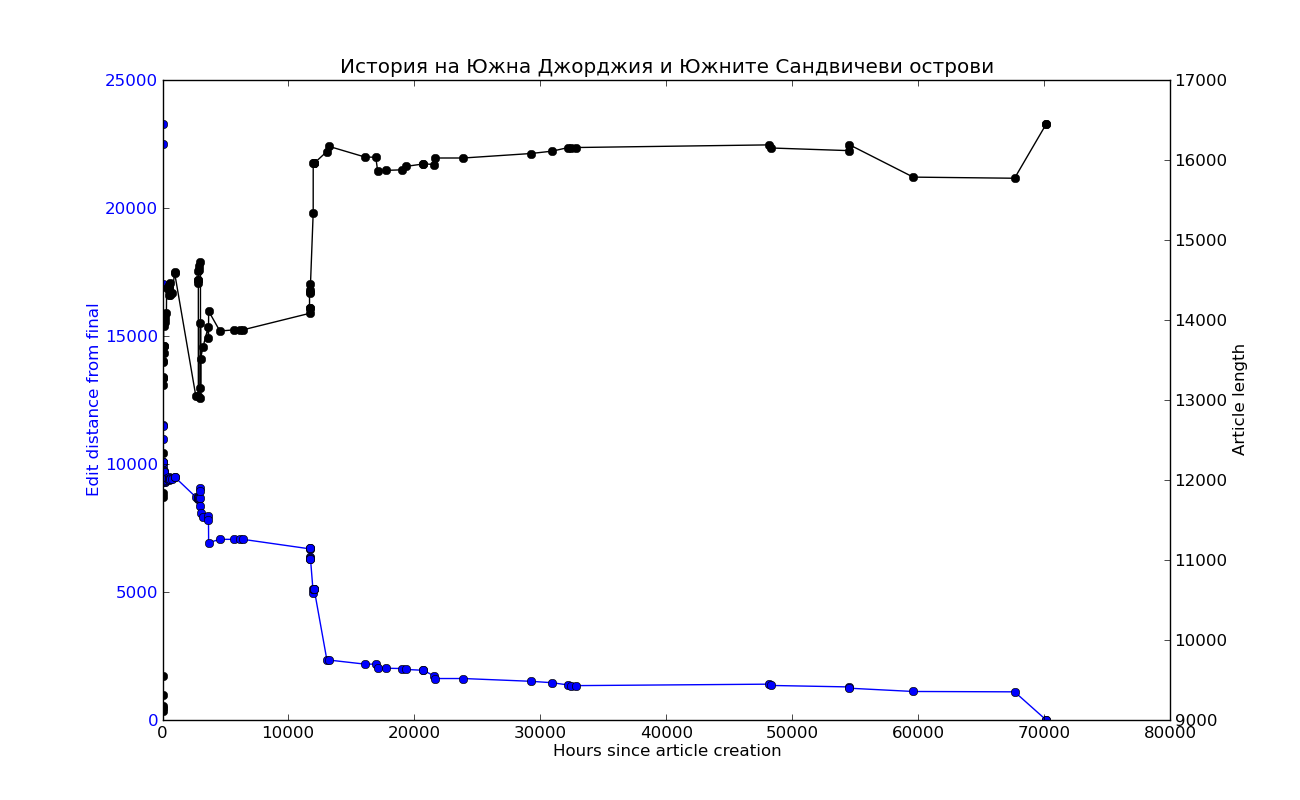
\includegraphics[width=\linewidth]{img/traj-classic/bg90882traj.png}
      \caption{\href{http://bg.wikipedia.org/wiki/index.php?curid=90882}{Bulgarian
      Wikipedia, Page ID 90882 (History of South Georgia and the South Sandwich Islands)}}
    \end{subfigure}
    \begin{subfigure}[b!]{0.6\linewidth}
      \centering
      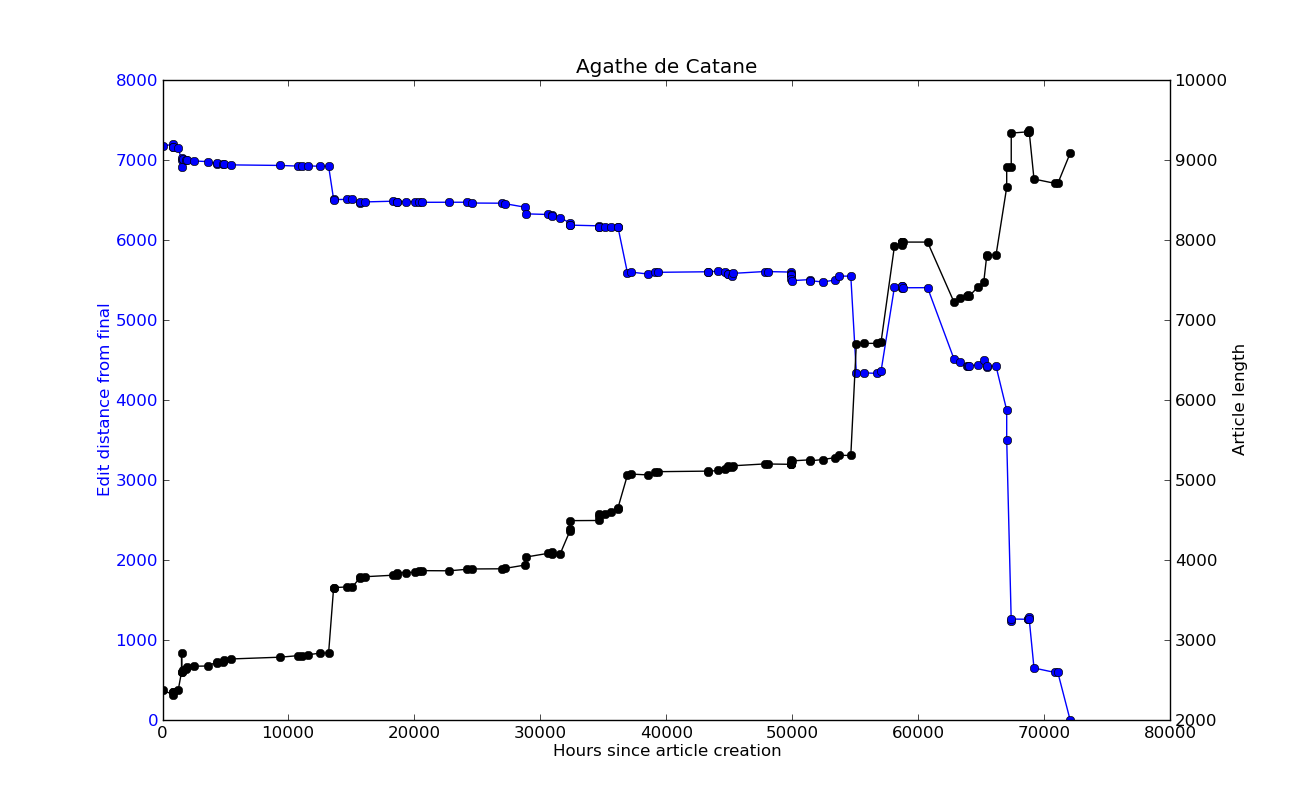
\includegraphics[width=\linewidth]{img/traj-classic/fr572796traj.png}
      \caption{\href{http://fr.wikipedia.org/wiki/index.php?curid=572796}{French
      Wikipedia, Page ID 572796 (Agatha of Catania)}}
    \end{subfigure}
  }\\
  \makebox[\linewidth][c]{
    \begin{subfigure}[b!]{0.6\linewidth}
      \centering
      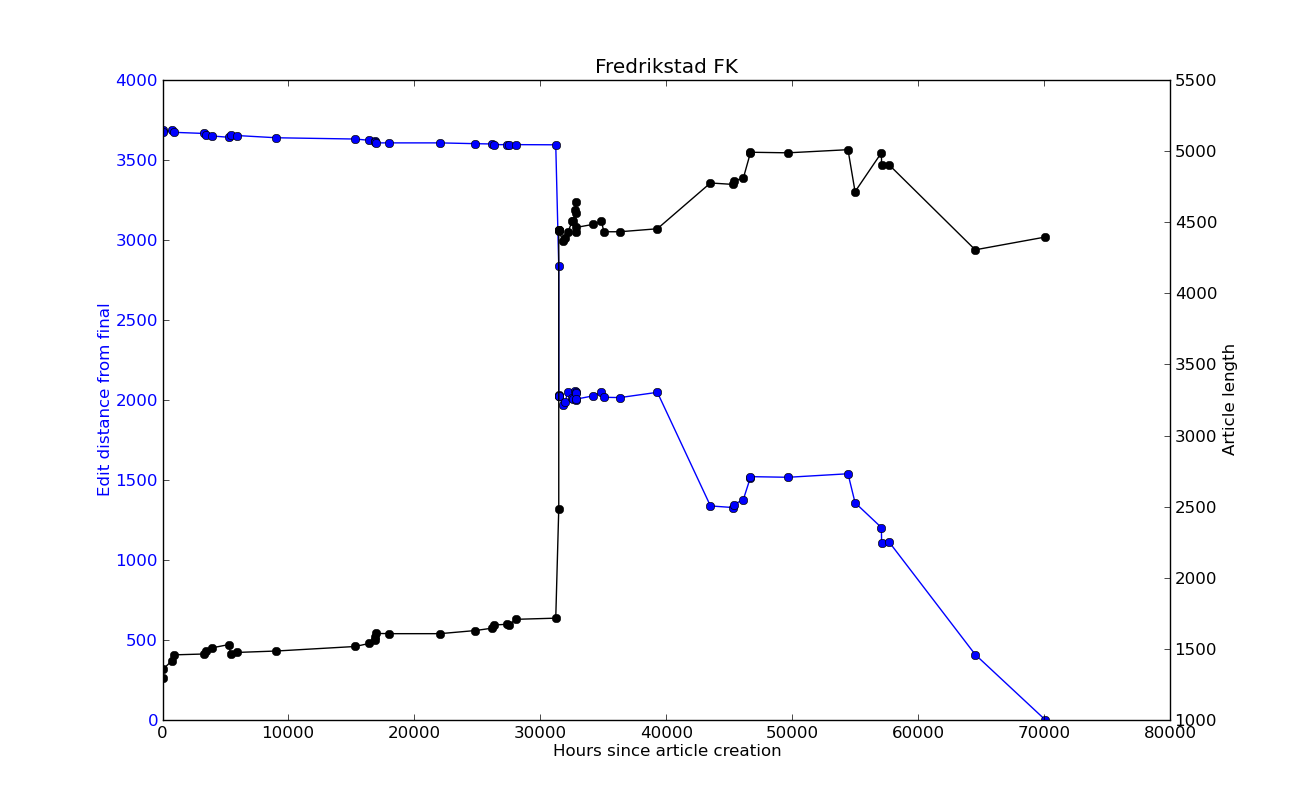
\includegraphics[width=\linewidth]{img/traj-classic/pl291709traj.png}
      \caption{\href{http://pl.wikipedia.org/wiki/index.php?curid=291709}{Polish
      Wikipedia, Page ID 291709 (Fredrikstad FK, a Norwegian football
      club)}}
      \label{fig:fredrikstad}
    \end{subfigure}
    \begin{subfigure}[b!]{0.6\linewidth}
      \centering
      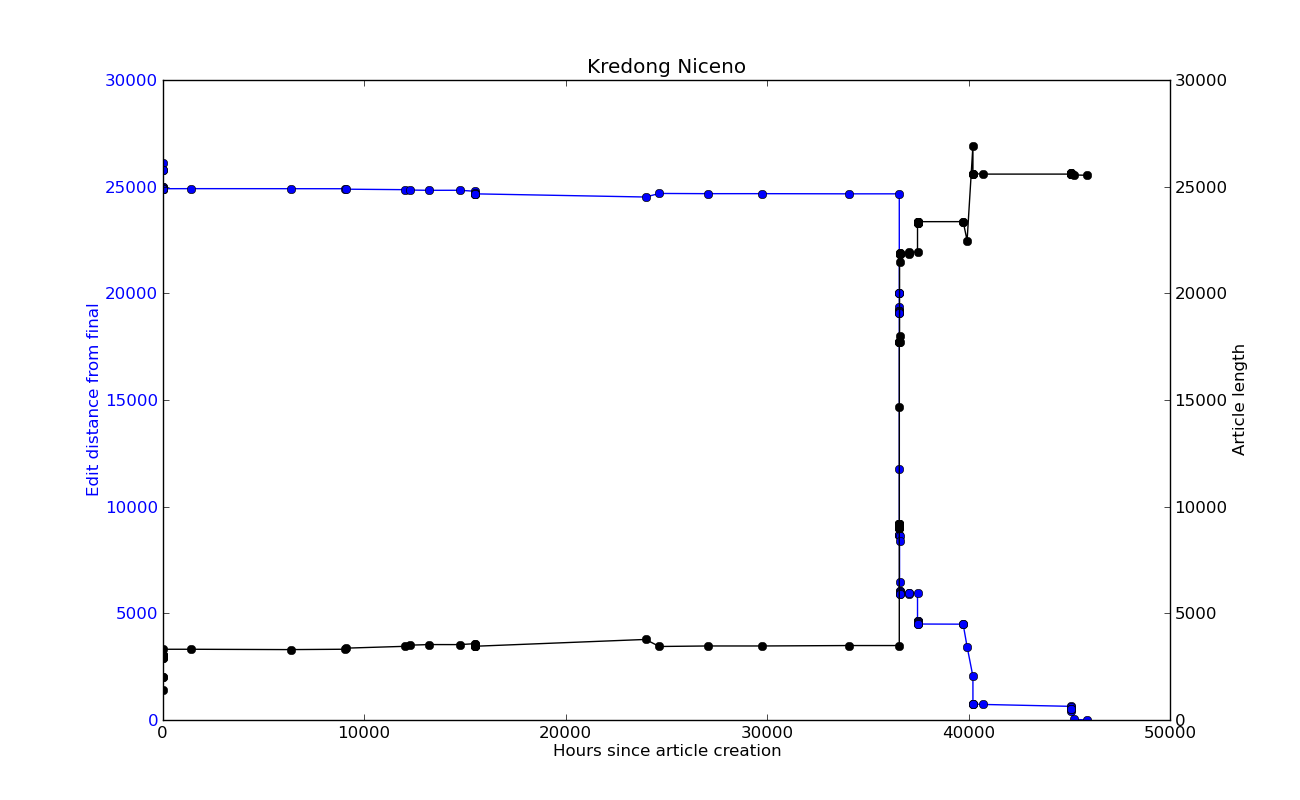
\includegraphics[width=\linewidth]{img/traj-classic/tl62286traj.png}
      \caption{\href{http://tl.wikipedia.org/wiki/index.php?curid=62286}{Tagalog
      Wikipedia, Page ID 62286 (The Nicene Creed)}}
      \label{fig:nicine-creed}
    \end{subfigure}
  }\\
  \makebox[\linewidth][c]{
    \begin{subfigure}[b!]{0.6\linewidth}
      \centering
      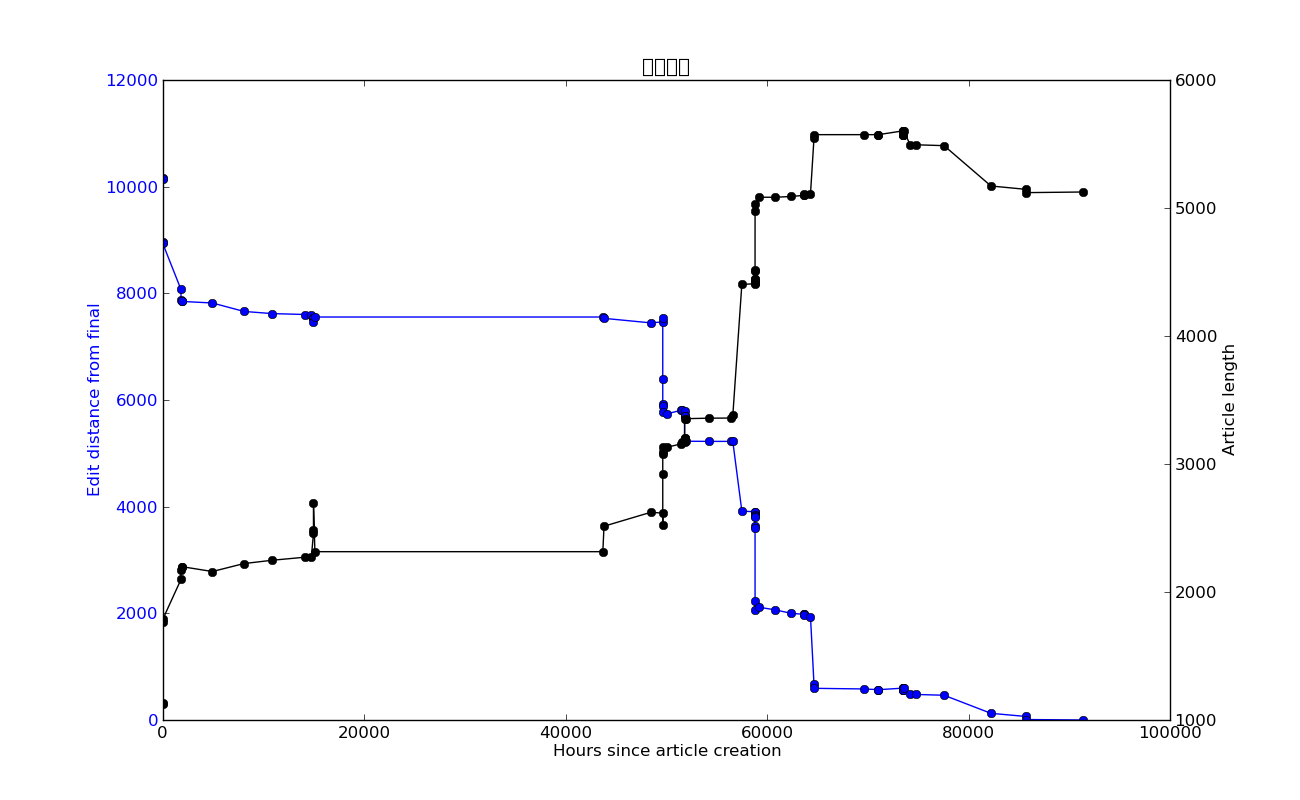
\includegraphics[width=\linewidth]{img/traj-classic/ja1611162traj.png}
      \caption{\href{http://ja.wikipedia.org/wiki/index.php?curid=1611162}{Japanese
      Wikipedia, Page ID 1611162 (The Tax Treaty)}}
      \label{fig:japanese-tax}
    \end{subfigure}
    \begin{subfigure}[b!]{0.6\linewidth}
      \centering
      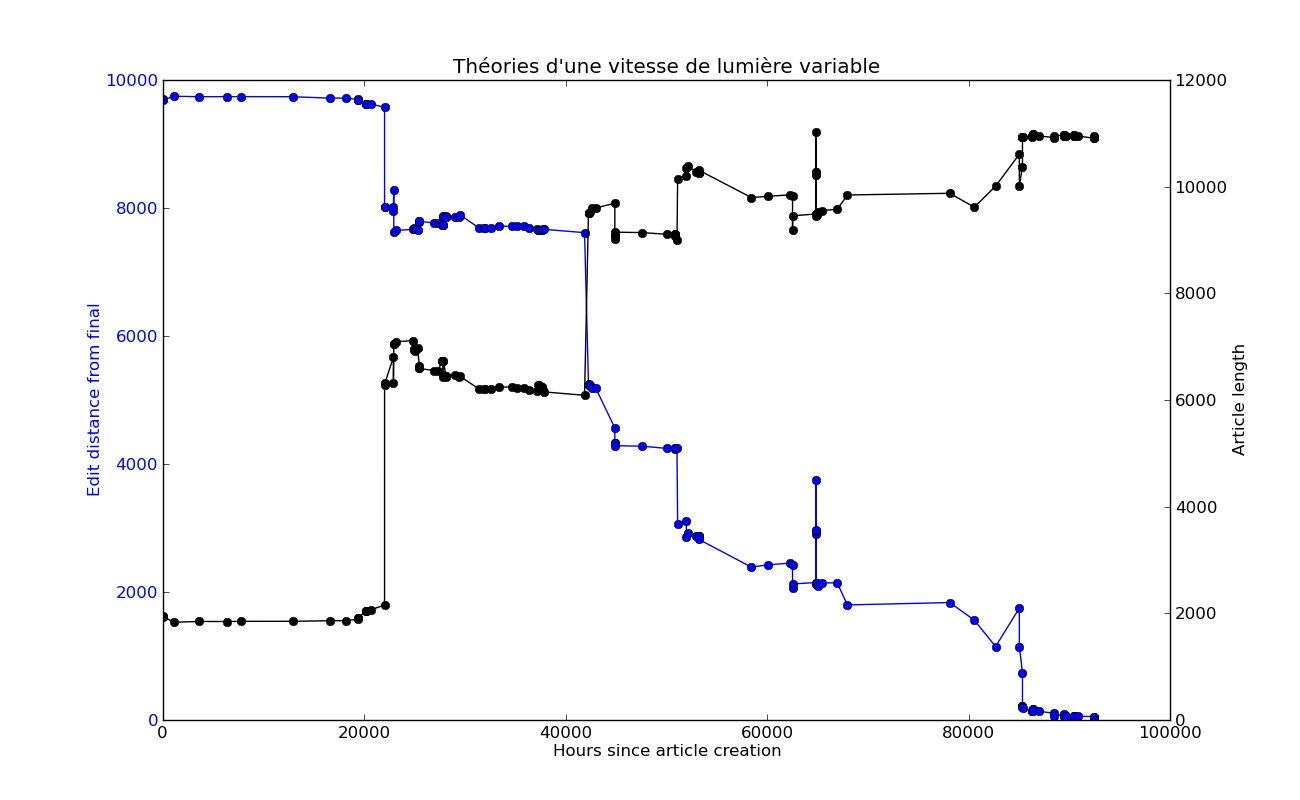
\includegraphics[width=\linewidth]{img/traj-classic/fr43937traj.png}
      \caption{\href{http://fr.wikipedia.org/wiki/index.php?curid=43937}{French
      Wikipedia, Page ID 43937 (Theories of a variable light speed)}}
      \label{fig:variable-light}
    \end{subfigure}
  }
  \caption{Simple trajectory graphs.}
\end{figure}

In the last of these simple trajectory graphs we find the first of our
notable features. Figure~\ref{fig:variable-light} shows a clear sign
of an undo operation at around 65,000 into the age of the article. We
see the black line take a steep ascent and immediate descent, showing
a quick enlargement and reduction of the article size. Since the same
spike can be seen in the blue line, we know that inserting this text
made the the article more different from the final version, and the
removed text brought us back. We can infer that the same text that was
added was the same as that which was removed. We find one of these
redo-undo edits
\href{http://fr.wikipedia.org/w/index.php?title=Th\%C3\%A9ories\_d\%27une\_vitesse\_de\_lumi\%C3\%A8re\_variable&diff=96659084&oldid=96654283}{in
  the wikipedia diff between revids 96659084 and 96654283}.

In contrast, the Phillipino article on the Nicene Creed
(Figure~\ref{fig:nicene-creed}) has a similar-shaped spike in it's
size. The event can be seen to occur just after 40000 hours. In this
case however, the trajectory line does not spike in turn. In this case
we can assume that the inserted spike shows an insertion of text that
remains in the article, and the deletion of text that is not
re-inserted before the article's current version.

These spikes are fairly obvious characteristics to identify on plots
such as these. However, we may also identify longer periods of
meandering away from and back towards the current version. Notice the
arced paths in figure~\ref{fig:fredrikstad}, spanning around 45000 to
55000 hours. Although the time frame is much larger than in the other
articles (10,000 hours $\approx$ 1 year 2 months), and multiple edits
occur in the meantime, we may also characterise the overall event as
an `undo' operation. It is more nuanced than others we have identified
so far (after the event the article is equally similar to the current
version, but smaller in size), but the effect is the same. The burden
is upon our model as to how to sufficiently characterise these
long-term discardations of useless inserted material.

We also may begin to notice that that edits may tend to cluster in
time, and that the articles may owe much of their content one-time
bursts of activity. The Japanese article on tax
(figure~\ref{fig:japanese-tax}), after an `undo'-shaped cluster of
edits at around 15000 hours, was not edited again for almost 3
years. The Tagalog and Polish articles (respectively the smallest and
largest articles discussed so far) gained most their content over just
a few days. 

However, many of the trajectories we trace bely a much stranger
history. Those in figure~\ref{fig:traj-bot} show a particular feature
a slow climb in both distance-from-final and size, before a sharp
drop. The shape is very common, and seems to describe an article which
becomes slowly bigger, before having the majority of it's content
deleted. In plotting the histories it seemed to occur very often, and
on further inspection we find each article to share two
characteristics -- they come from small Wikipedias, and the majority
of the edits are made by bots.\footnote{We can see from the usernames on the
right-hand side graphs in figure~\ref{fig:traj-bot} that they are bots
-- there is a special bot `flag' to be raised in the user profile of
bots, but it is also traditional for the bot to be also be given an
identifying name.\cite{wiki-bot-policy}}
 
\begin{figure}
  \label{fig:traj-bot}
  \centering
  \makebox[\linewidth][c]{
    \begin{subfigure}[b!]{1.2\linewidth}
      \centering
      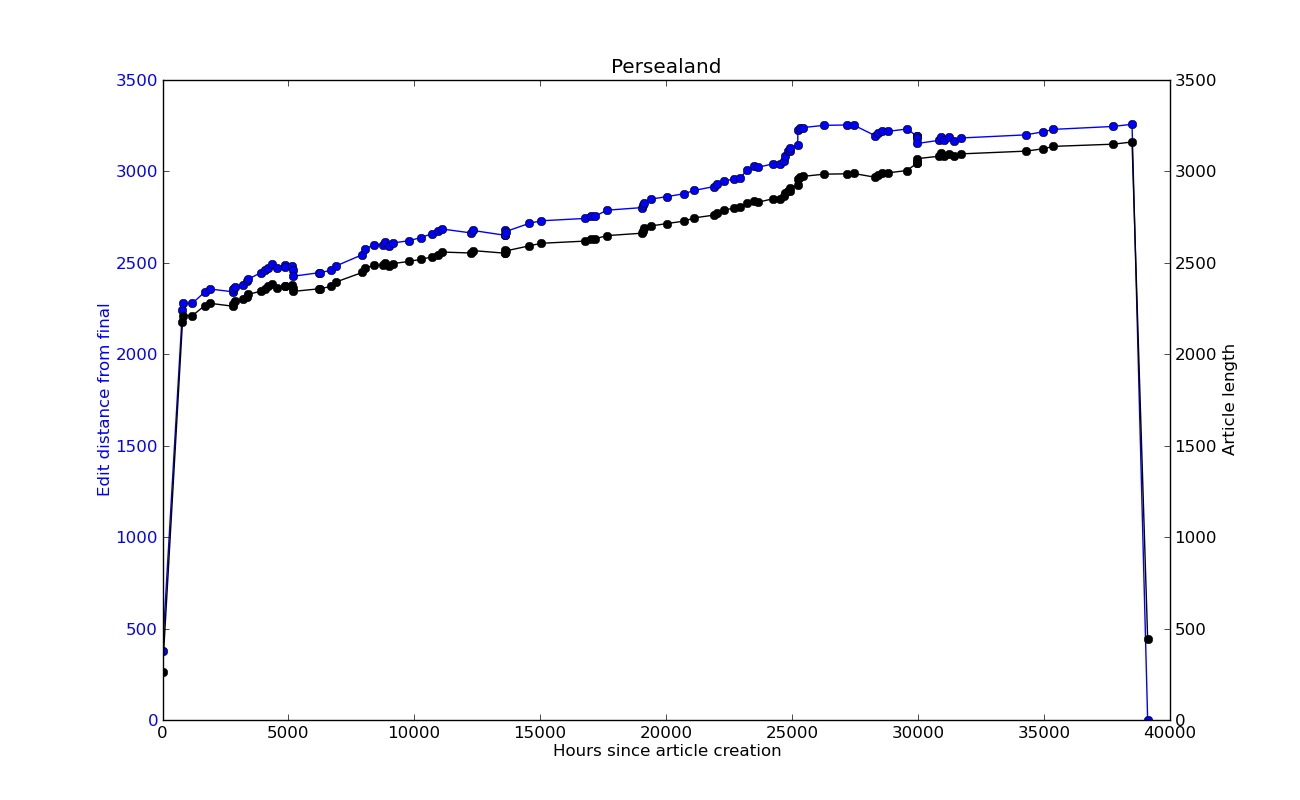
\includegraphics[width=0.45\linewidth]{img/traj-bot/ang7120traj.png}
      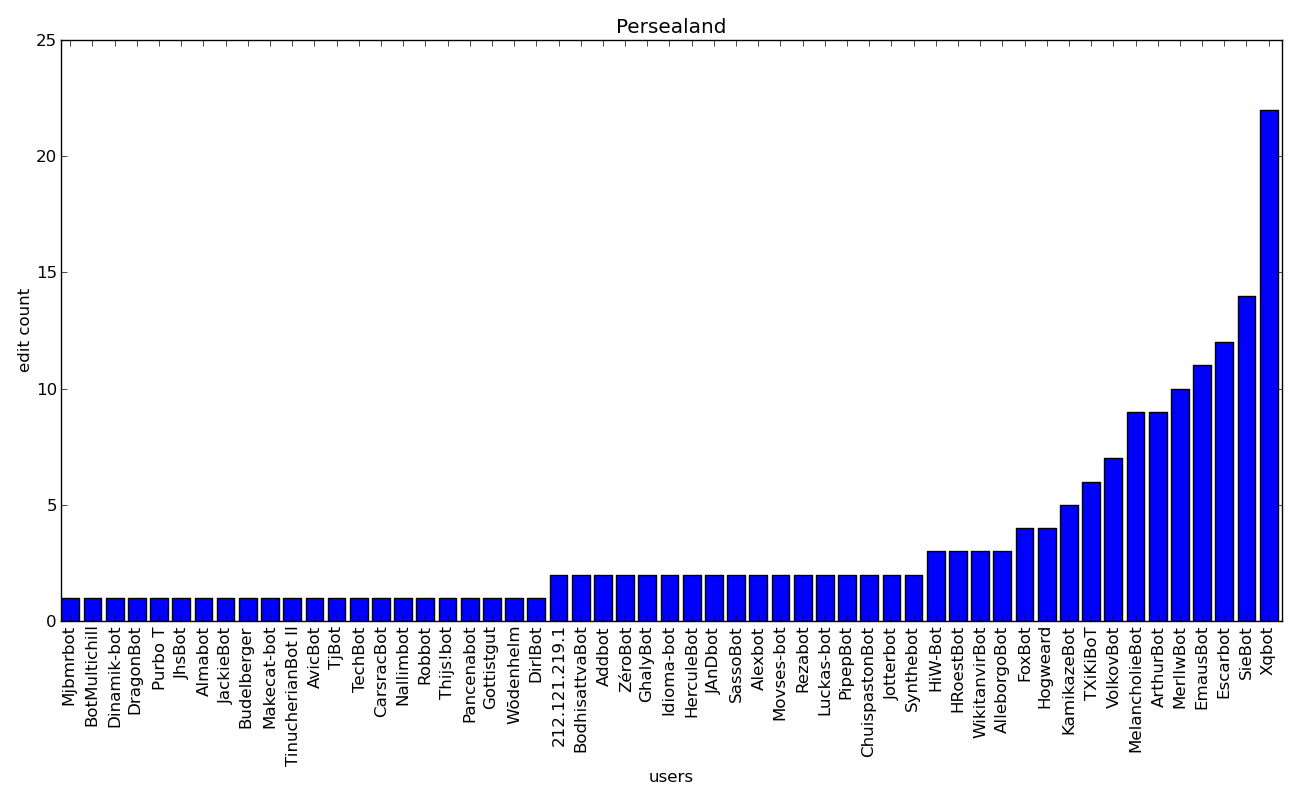
\includegraphics[width=0.45\linewidth]{img/traj-bot/ang7120users.png}
      \caption{\href{http://ang.wikipedia.org/wiki/index.php?curid=7120}{Anglo-Saxon
      Wikipedia, Page ID 7120 (Persia)}}
    \end{subfigure}
  }\\
  \makebox[\linewidth][c]{
    \begin{subfigure}[b!]{1.2\linewidth}
      \centering
      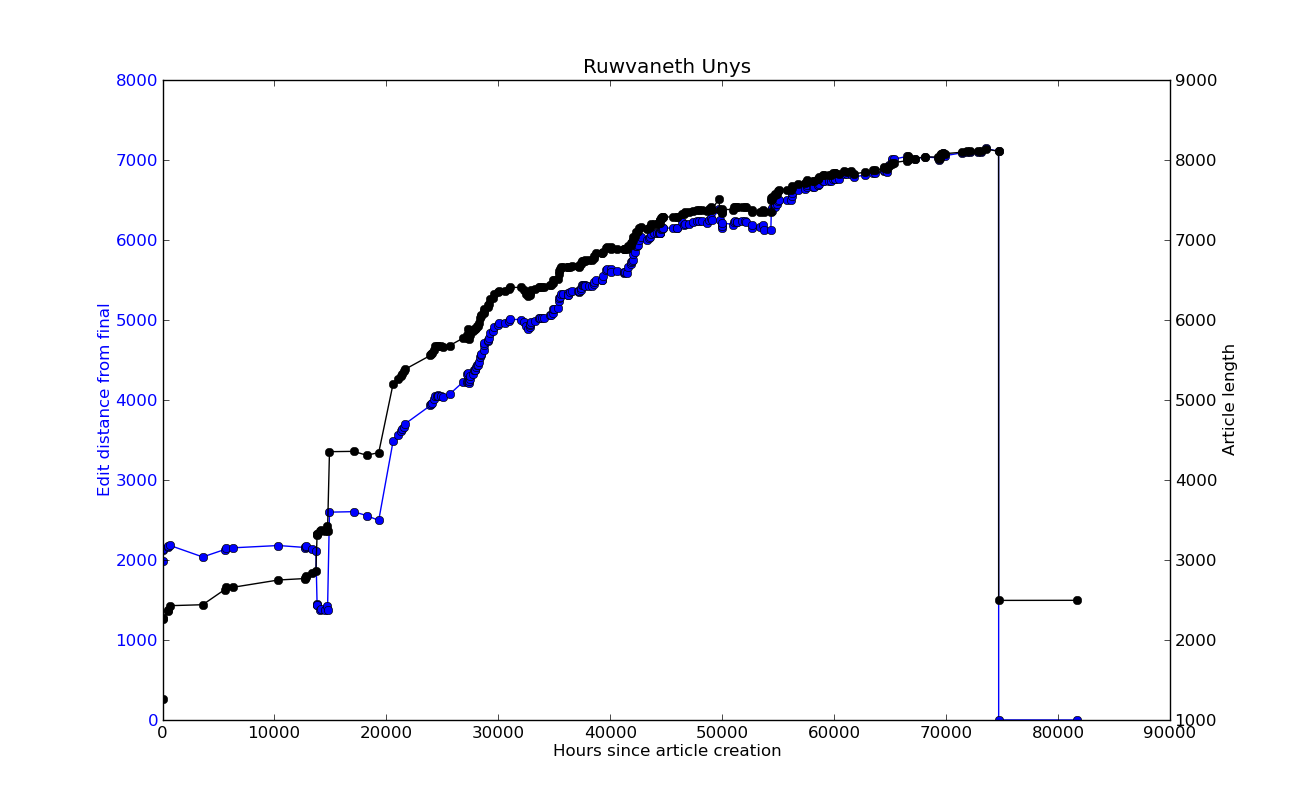
\includegraphics[width=0.45\linewidth]{img/traj-bot/kw736traj.png}
      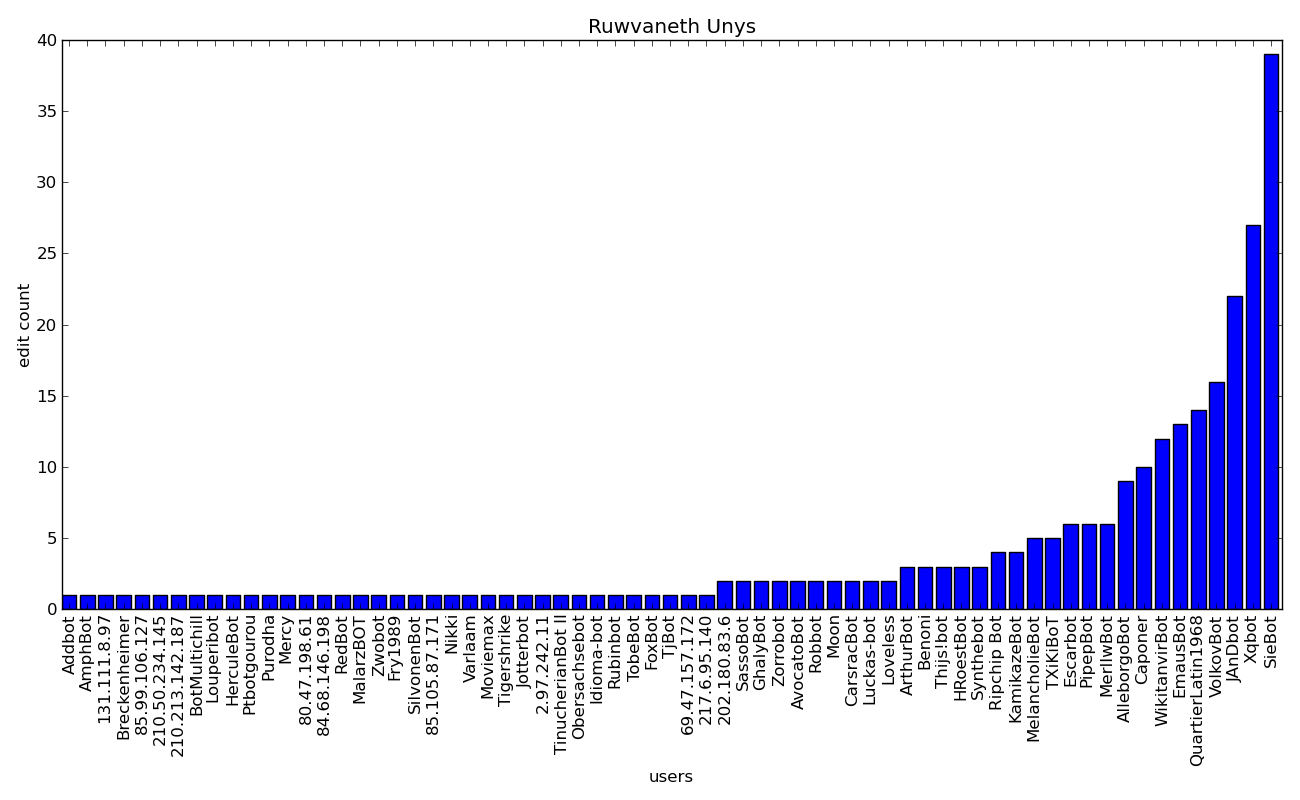
\includegraphics[width=0.45\linewidth]{img/traj-bot/kw736users.png}
      \caption{\href{http://kw.wikipedia.org/wiki/index.php?curid=736}{Cornish
      Wikipedia, Page ID 726 (United Kingdom)}}
    \end{subfigure}
  }\\
  \makebox[\linewidth][c]{
    \begin{subfigure}[b!]{1.2\linewidth}
      \centering
      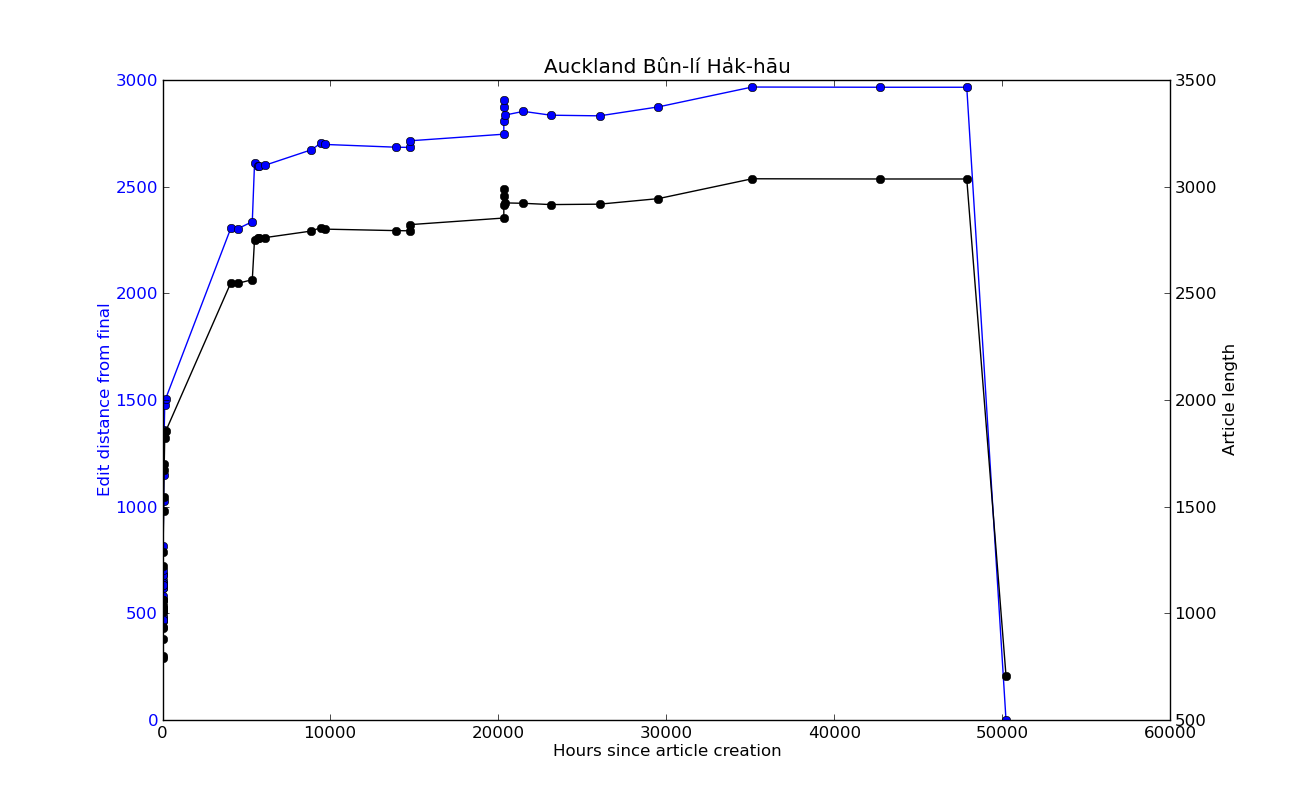
\includegraphics[width=0.45\linewidth]{img/traj-bot/zh-min-nan10733traj.png}
      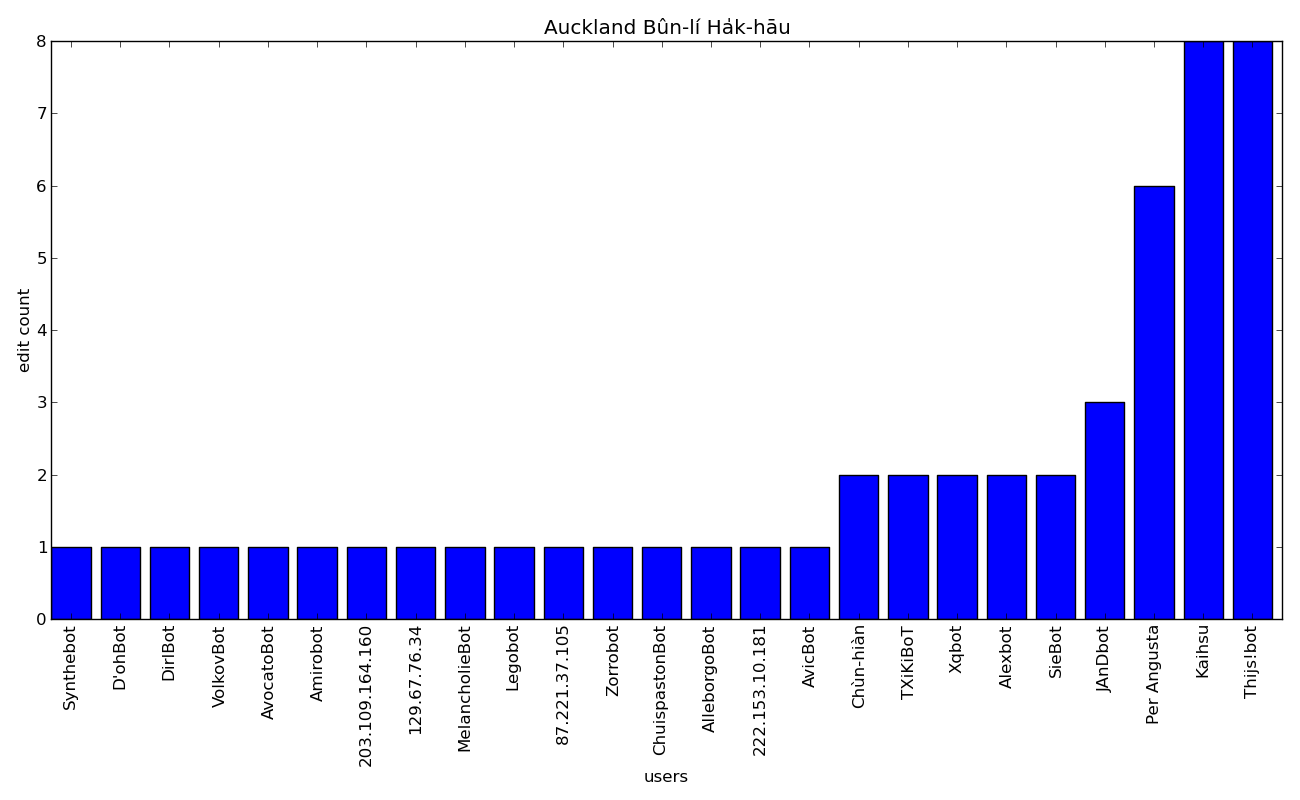
\includegraphics[width=0.45\linewidth]{img/traj-bot/zh-min-nan10733users.png}
      \caption{\href{http://zh-min-nan.wikipedia.org/wiki/index.php?curid=10733}{Min Nan
      Wikipedia, Page ID 10733 (Auckland Grammar School)}}
    \end{subfigure}
  }\\
\caption{Trajectory graphs showing bot editing characteristics.}
\end{figure}

The explanation is in the articles' histories. In each one, we find a
single large deletion event, ocurring any time after early 2013. With
a little digging, we find the origin of the act to be a Wikimedia
project that aims to `migrating interlanguage wiki links from
individual articles into a central database to ease
maintenance',\cite{wiki-interwikilinks} see
figure~\ref{traj-bot-explanation} for evidence of just one of these
events. Each wikipedia article is rendered to the right of a language
bar that links that article to its counterpart in various
languages. Once coded into each article manually, that data is now
stored in and served from a central source.\cite{wiki-blog-onwikidata}
The move gives us strange results for this project -- for small
articles, the loss of these hard-coded links constitutes a gutting of
its majority content. By our measurements, in these circumstances,
this act of housekeeping is a momentous event in the history of small
articles.

\begin{figure}
  \label{fig:traj-bot-explanation}
  \centering
  \makebox[\linewidth][c]{
    \begin{subfigure}[b!]{1.2\linewidth}
      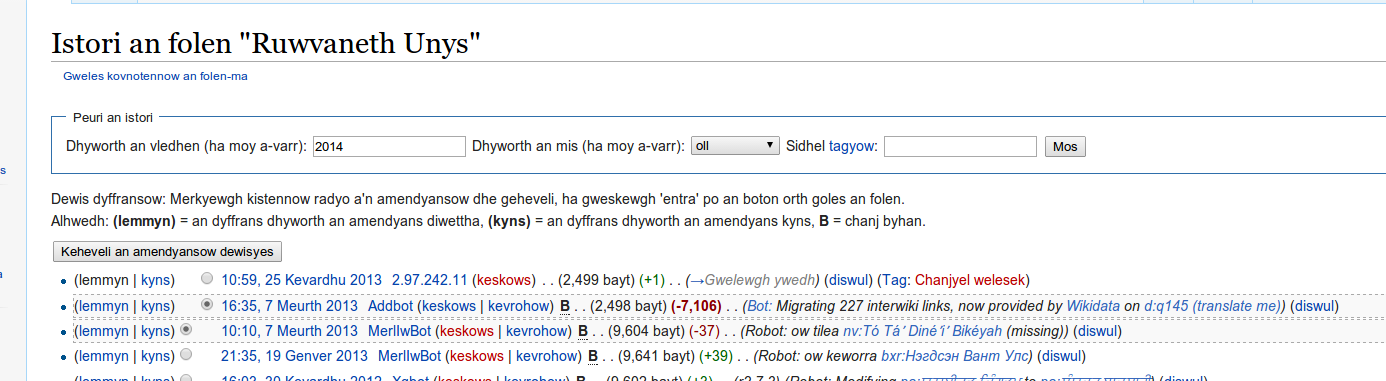
\includegraphics[width=1\linewidth]{img/traj-bot/botmigration.png}
      \caption{Migration event in article history (16:35, 7 March 2013)}
    \end{subfigure}
  }\\
  \makebox[\linewidth][c]{
    \begin{subfigure}[b!]{1.2\linewidth}
      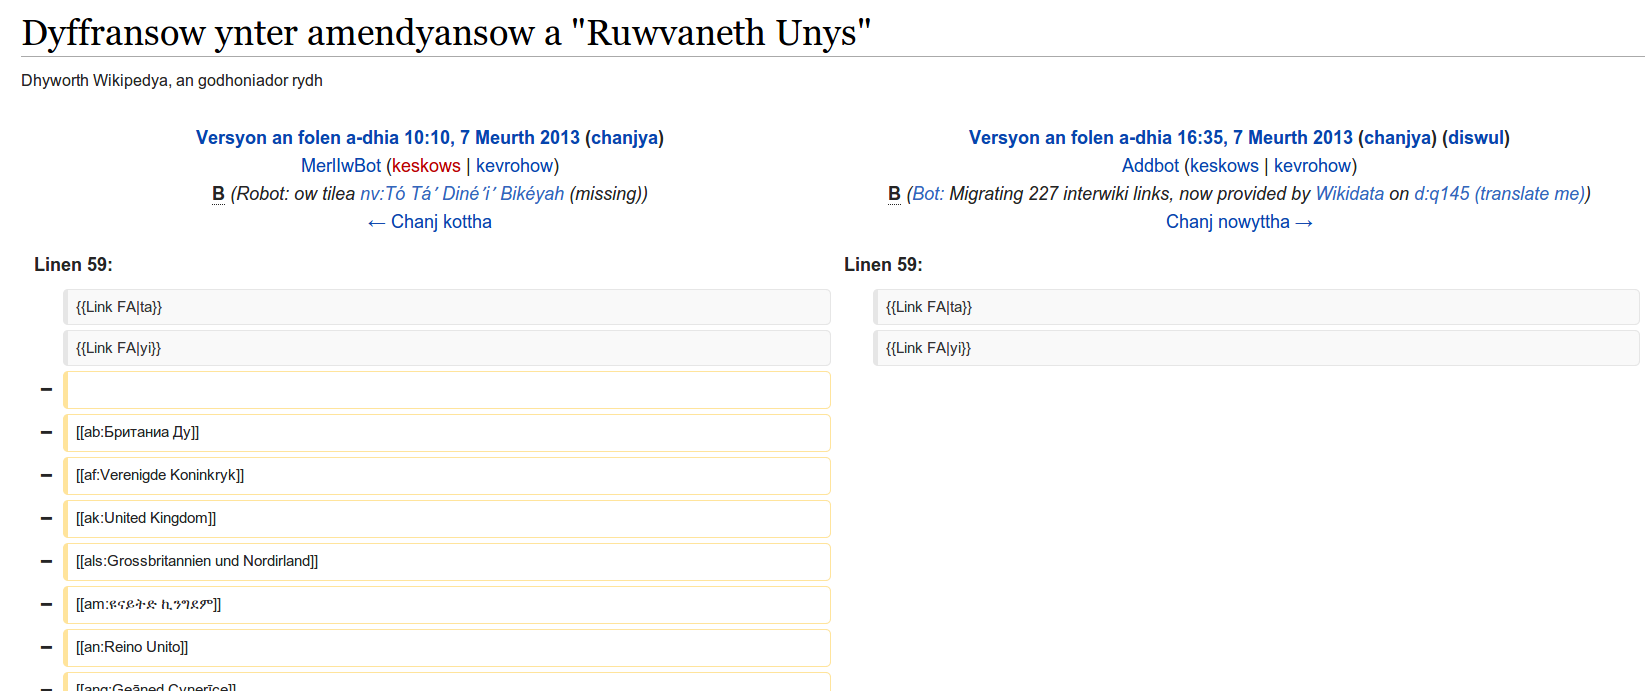
\includegraphics[width=1\linewidth]{img/traj-bot/botdiff.png}
      \caption{The Wikipedia diff for the migration event}
    \end{subfigure}
  }
\caption{Screenshots showing automated migration of inter-language links.}
\end{figure}

How do we characterise this? In this case the `article', as such, is
unchanged. Indeed the rendered page is identical before and after the
link cull. We may think to ignore bot edits to a page, but how do we
distinguish between the adding and deletion of these language links
from meaningful changes to content? We may distinguish from, say,
useful spell-checking bots by means of a simple text regex (inter-wiki
links always have the same form), but we may not as easily distinguish
language-bar links from inline ones -- those that may link to related
articles, rather than mirror articles, widening knowledge rather than
offering what may merely be a translation of the original
article.

IS THERE MORE EXAMPLE OF WEIRD WIKI STUFF MESSING UP RESULTS?

PLOT DISTRIBUTION OF EDIT NUMBER ON EN, DE, IT

PLOT DISTRIBUTION OF SPECIES OF TEXT 

